\appendix
\renewcommand{\thesection}{A.\arabic{section}}
\renewcommand{\thesubsection}{A.\arabic{section}.\arabic{subsection}}
\renewcommand{\thesubsubsection}{A.\arabic{section}.\arabic{subsection}.\arabic{subsubsection}}
\renewcommand\thefigure{A.\arabic{section}.\arabic{figure}}   
\appendixpage
\addappheadtotoc
\section{Glosario y abreviaciones}
\printglossary
\printglossary[type=\acronymtype, title=Abreviaciones]
\section{Formularios}
\subsection{Registro de movimiento}
\begin{figure}[H]
	\caption{Formulario de  registro de movimiento (Blanco)}
	\label{fig:frmWhiteMov}
	\centering
	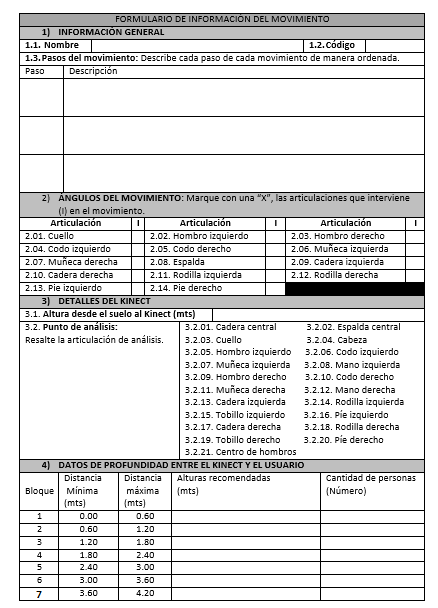
\includegraphics[width=420px,height=520px]{graphics/frm-mov.PNG} \\
	\textbf{Fuente:} Elaborado por el autor de tesis
\end{figure}
\subsubsection{Movimiento de cheerleaders}
\subsubsection{Movimiento de taekwondo}
\subsubsection{Movimiento de tenis de mesa}
\subsection{Programaci\'on de rutina para captura de datos}
\begin{figure}[H]
	\caption{Formulario de  registro de movimiento (Blanco)}
	\label{fig:frmWhiteRout}
	\centering
	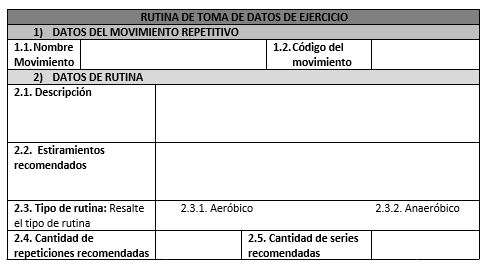
\includegraphics[width=420px,height=250px]{graphics/frm-rutina.PNG} \\
	\textbf{Fuente:} Elaborado por el autor de tesis
\end{figure}
\section{Hojas de observaciones}
\subsection{Observaciones de profundidad entre usuario y Kinect}
\begin{figure}[H]
	\caption{Registro de datos de profundidad (Blanco)}
	\label{fig:PObvDeep}
	\centering
	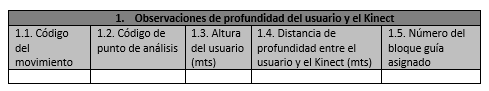
\includegraphics[width=420px,height=120px]{graphics/hObv-ProfundidadKinect.PNG} \\
	\textbf{Fuente:} Elaborado por el autor de tesis
\end{figure}
\subsubsection{Ejemplo de observaciones}

